%%%%
%% Design :: Sequence Diagrams
%%%
\section{Sequence Diagrams}
\label{sec:sequence_diagrams}

Within the previous \nameref{sec:use_case} section a number of key, generic 
functions were identified. In order for a sequence diagram to be developed, 
the generic functions will be converted into a set of objects and interactions.
Each of the objects and interactions will eventually form the classes that will 
be used to build the system. Therefore a sequence diagram can be described as 
a ``way of describing a journey through a system'' \citep{lunn03}.

The two sequence diagrams that will be described within this section focus upon 
submitting a clue and solving a clue.


%%%
%% Design :: Sequence Diagrams :: Submitting a Clue
%%
\subsection{Submitting a Clue}
\label{sub:submitting_a_clue}

Figure \ref{fig:submit_clue_sequence} illustrates a user sending data to the 
web service (servlet). Within this diagram a number of key elements such as how
a clue will be solved have been removed. This is the ensure that the diagram is 
as simple as possible, as this diagram will only be focusing upon how a user 
sends and receives data. 

The \nameref{sub:solving_a_clue} subsection on page 
\pageref{fig:submit_clue_sequence} describes in detail how a solver will solve 
the clue.

To simplify the diagram the user is submitting a `block' of data, which in fact 
would be the three main parameters --- the clue, the solution length and the 
solution pattern. This has been shown upon the diagram as a `block' of data, 
because all three parameters will be sent to the system at the same time.

Once the data has arrived at the servlet, the data will be validated. If the 
data is deemed to be invalid, the servlet will send an error response back, 
finishing the current instance.

If the data is deemed to be valid, then the system will try to categorise the 
clue, and solve the clue using the required solver(s). This is will be discussed
in more detail in the \nameref{sub:solving_a_clue} subsection on page 
\pageref{fig:submit_clue_sequence}.

Once a set of solutions have been generated, the the in-memory set will be 
converted to either JSON or XML depending upon the client's request. Once 
converted the data is returned as part of the response, satisfying the client's
request.

\begin{figure}[H]
  \centering
  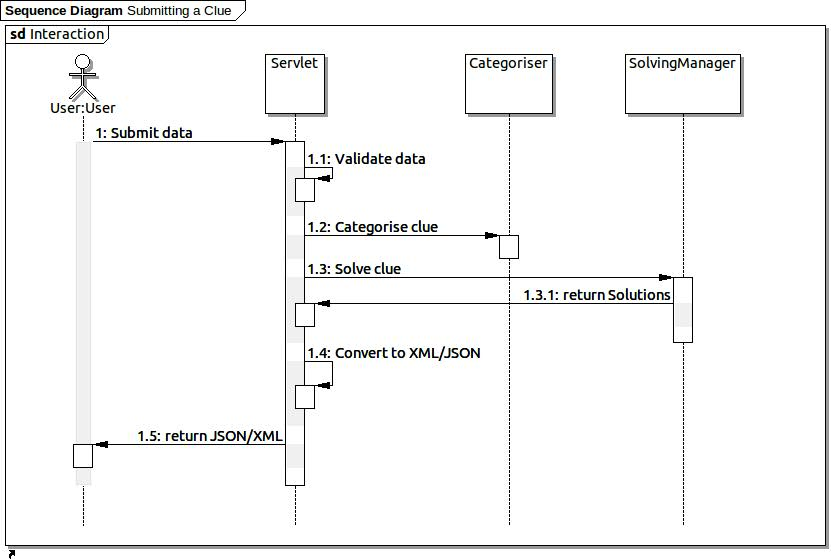
\includegraphics[width=0.9\textwidth]{sequence/submitting_a_clue.jpg}
  \caption{Sequence digram illustrating a user submitting a clue}
  \label{fig:submit_clue_sequence}
\end{figure}


%%%
%% Design :: Sequence Diagrams :: Solving a Clue
%%
\subsection{Solving a Clue}
\label{sub:solving_a_clue}

Figure \ref{fig:solving_clue_sequence} illustrates how a given clue will be 
solved. This sequence diagram assumes that valid data has been passed to the 
`SolvingManager'. This process was described in the previous subsection entitled
`\nameref{sub:submitting_a_clue}' on page \pageref{sub:submitting_a_clue}.

The `SolvingManager' object will manage the process of solving a given clue. In 
order to do this it will have to house several processes, including distributing
the clue out to one or more solvers, and merging all results.

Figure \ref{fig:solving_clue_sequence} illustrates the distributing and solving
of the clue as a synchronous process, however this was used for illustrative
purposes only. The system will in fact distribute and solve the clue upon an
asynchronous basis. This will mean that each solver will be running at the same 
time, and thus reducing the total amount of time needed to solve the clue.

The system will wait however, for all solvers to finish, ensuring that all 
solutions can be returned to the user. The merging of the results will simply 
remove any duplicate solutions, upon a first come basis. So if a solution is 
already in the list, it will not be re-added because a different solver has 
managed to find the same solution.

Finally the confidence ratings will be adjusted. The adjustments are made upon 
a number of factors, and were described in figure \ref{fig:results_activity} on
page \pageref{fig:results_activity}.

\begin{figure}[H]
  \centering
  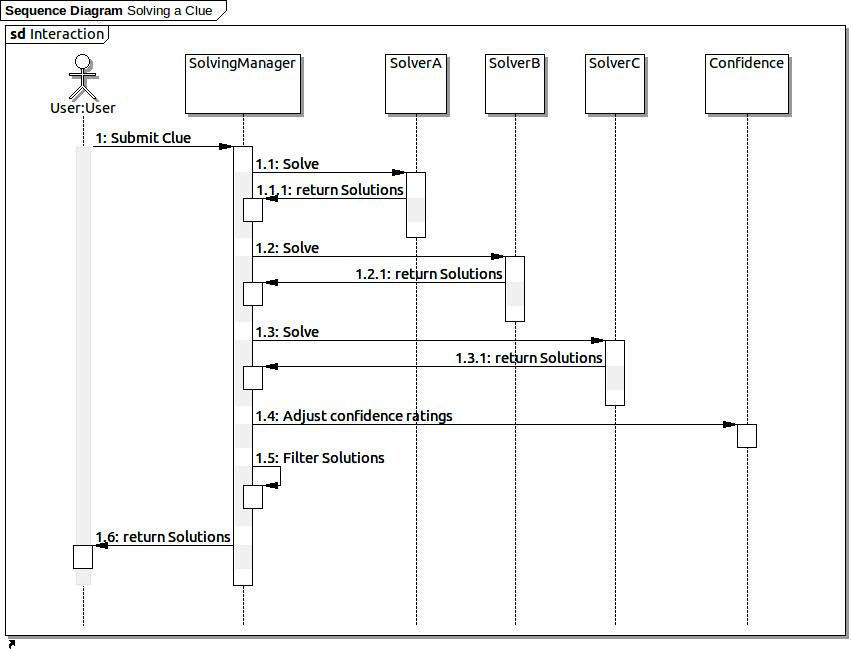
\includegraphics[width=0.9\textwidth]{sequence/solving_a_clue.jpg}
  \caption{Sequence digram illustrating the system solving a clue}
  \label{fig:solving_clue_sequence}
\end{figure}
